\documentclass{siproblemset}

\usepackage{graphicx}
\usepackage{multicol}
\usepackage{xcolor}
\usepackage{mathtools}

% SI Session Information
\course{MTH 1321}
\sessionnum{PT4}
\sessiondate{4/28/20}

% Worksheet Information
\title{Practice Test \#4}
\sections{Chapter 5}
\withnamespace

\definecolor{darkred}{RGB}{110,0,0}

%\debugmode

\begin{document}
    \maketitle
    
    \begin{center}
        \framebox{
            \begin{minipage}{\textwidth}
                \begin{center}
                    \textbf{When completing this practice test, do your best to mimic the test environment:}
                \end{center}
                \begin{enumerate}
                    \item Do not use a calculator.
                    \item Try not to use your notes.
                    \item Time yourself, make sure you are completing the problems at a comfortable pace. Remember that you will only get 55 mins for the actual exam (with fewer questions of course).
                \end{enumerate}
                {\centering \color{blue}When you have finished the practice test, \\check the ``Modules'' section on Canvas for the answer key.\\}
            \end{minipage}
        }
    \end{center}

    \begin{align*}
        \sum_{j=1}^{n}k &= kn \\
        \sum_{j=1}^{n}j &= \dfrac{n(n+1)}{2} = \dfrac{n^2}{2} + \dfrac{n}{2} \\
        \sum_{j=1}^{n}j^2 &= \dfrac{n(n+1)(2n+1)}{6} = \dfrac{n^3}{3} + \dfrac{n^2}{2} + \dfrac{n}{6} \\
        \sum_{j=1}^{n}j^3 &= \dfrac{n^2(n+1)^2}{4} = \dfrac{n^4}{4} + \dfrac{n^3}{2} + \dfrac{n^2}{4} 
    \end{align*}
    
    \newpage

    \begin{multipartquestion}
        \frq{On the graph below, add rectangles representing $L_3$ on $[-1,5]$. Then, compute the $L_3$ approximation on this interval.}
        \includegraphics[width=0.7\linewidth]{img/pt4-draw-rectangles}
        
        \frq{On the graph below, add rectangles representing $M_3$ on $[-1,5]$. Then, compute the $M_3$ approximation on this interval.}
        \includegraphics[width=0.7\linewidth]{img/pt4-draw-rectangles}
        \newpage
        
        \frq{On the graph below, add rectangles representing $R_3$ on $[-1,5]$. Then, compute the $R_3$ approximation on this interval.}
        \includegraphics[width=0.7\linewidth]{img/pt4-draw-rectangles}
    \end{multipartquestion}

    \begin{multipartquestion}
        \frq{Find a formula for $R_n$, for the following function on the given interval.}
        $$f(x)=3x-1~~[-1,2]$$
        \Normalsp
        \frq{Using your formula for $R_n$ above, compute $\lim\limits_{n\to\infty}R_n$.}
        \tinysp
        \frq{What does your answer to part (b) represent?}
    \end{multipartquestion}
    \newpage
    
    \begin{multipartquestion}
        Let $A(x)=\int_{0}^{x}f(t)dt$. The graph of $f(x)$ is given below.
        
        \begin{center}
            \includegraphics[width=0.7\linewidth]{img/pt4-integral-graph}
        \end{center}
        
        \mcq[3]{Compute each of the following.}{
            \task $A(0)$
            \Tinysp
            \task $A(3)$
            \task $A(5)$
            \task $A(10)$
            \task $A'(4)$
            \task $A'(6)$
        }
        \Tinysp
    
        \frq{For what \underline{value(s)} of $x$ does $A(x)$ have a local maximum or minimum on $[0,10]$?}
        \smallsp
        
        \frq{Find the \underline{coordinate(s)} of each maximum and minimum of $A(x)$ on $[0, 10]$.}
        \smallsp
        
        \frq{Find a formula for $A(x)$ on $[2,3]$.}
    \end{multipartquestion}
    \newpage

    \mcq{Compute the following integrals, given $\int_1^6f(x)\dd x=8$, $\int_1^2f(x)\dd x=2$, and $\int_1^6g(x)\dd x=-5$.}{
        \task $\int_1^6\paren{f(x)+g(x)}\dd x$
        \smallsp
        \task $\int_1^63g(x)\dd x$
        \smallsp
        \task $\int_6^1f(t)\dd t$
        \smallsp
        \task $\int_2^6f(x)\dd x$
        \smallsp
        \task $\int_1^6\paren{3f(x)-2g(x)}\dd x$
        \smallsp
    }
    \newpage
    
    \frq{Find the exact value of the signed area between the curve $f(x)$ and the $x$-axis for $1\leq x\leq e$ where $f(x)=\dfrac{1}{16}x^2-\dfrac{x+1}{x}$. }
    \hugesp
    
    \frq{Find the \underline{total} area between the $x$-axis and $f(x)=x^2-x$ on $[0,2]$.}
    \newpage
        
    \begin{multipartquestion}
        The graph of $y=2^{-x}$ is shown below.
          \begin{center}
            \mbox{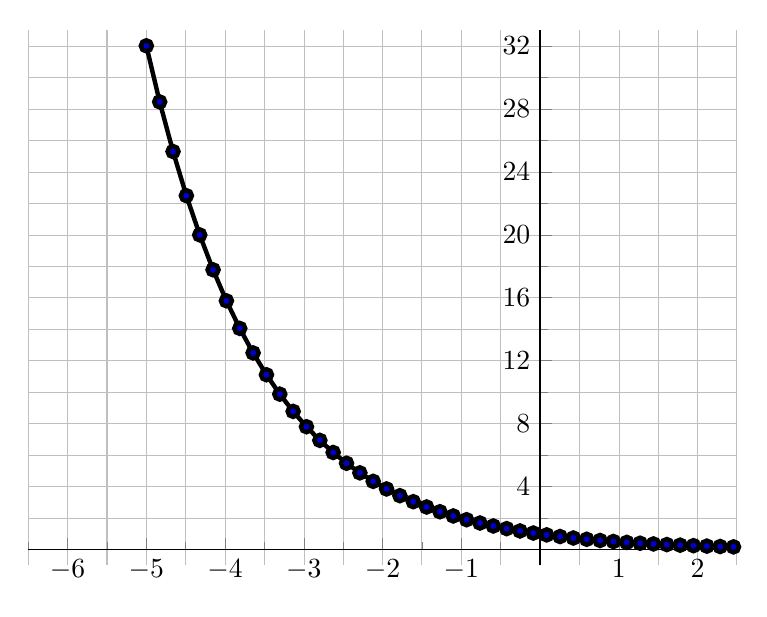
\begin{tikzpicture}[baseline=(current bounding box.north)]
                \begin{axis}[
                x=1cm,
                y=0.20cm,
                ytick distance=4,
                xmin=-6.5,
                xmax=2.5,
                ymin=-1,
                ymax=33,
                grid=both,
                major grid style={line width=.2pt,draw=gray!50},
                minor tick num=1,
                axis x line*=middle,
                axis y line*=middle,
                every axis plot/.append style={ultra thick},
                samples=60
                ]
                \addplot+[black] {2^(-x)};
                \end{axis}
                \end{tikzpicture}}
        \end{center}
        \frq{Estimate the area between the graph of $y=2^{-x}$ and the $x$-axis from $x=-5$ to $x=1$ by finding $L_3$, the left-endpoint approximation with 3 subintervals of equal width. Draw the rectangles you use on the graph above.}
        \Normalsp
        \frq{Considering the rectangles you drew, is the left-endpoint approximation an overestimate or underestimate? What about if we did the right-endpoint approximation instead?}
        \Smallsp
    \end{multipartquestion}
    \newpage
    
    \begin{multipartquestion}
        Use the graph of $f$ below to compute the following definite integrals.
        \begin{center}
            \mbox{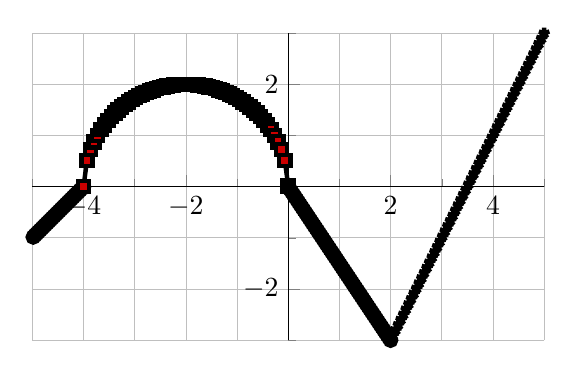
\begin{tikzpicture}[baseline=(current bounding box.north)]
                \begin{axis}[
                x=0.65cm,
                y=0.65cm,
                xmin=-5,
                xmax=5,
                ymin=-3,
                ymax=3,
                grid=both,
                major grid style={line width=.2pt,draw=gray!50},
                minor tick num=1,
                axis x line*=middle,
                axis y line*=middle,
                every axis plot/.append style={ultra thick},
                samples=60
                ]
                \addplot+[black, domain=-6:-4] {x+4};
                \addplot+[black, domain=-4:0] {sqrt(4-(x+2)^2)};
                \addplot+[black, domain=0:2] {-3/2*x};
                \addplot+[black, domain=2:5] {2*x-7};
                \end{axis}
                \end{tikzpicture}}
        \end{center}
        \frq{$\int_{-4}^{2}f(x)\text dx$}
        \tinysp
        \frq{$\int_{5}^{3}f(x)\text dx$}
        \tinysp
        \frq{$\int_{0}^{2}|f(x)|\text dx$}
        \tinysp
        \frq{$\int_{-2}^{2}3f(x)\text dx$}
        \tinysp
    \end{multipartquestion}

    \frq{Find $y(t)$ when $\dddf[y]{t}=(3t+2)^3$, $y(0)=1$.}
    \newpage
    
    \mcq{Beginning at $t=0$, a particle moves in a straight line with velocity $v(t)=3t-6$ \si{\meter/\second}.}{
        \task  Find the displacement of the particle after 8 s.
        \task  Find the distance traveled after 8 s.
    }
    \newpage
    
    
    \mcq{Evaluate.}{
        \task $\int_{1}^{e}\left(x+\frac1x\right)\text dx$
        \Smallsp
        \task $\int_{3}^{5}e^{-4t}\text dt$
        \Smallsp
        \task $\int_{0}^{\pi}\cos(2s)\text ds$
        \Smallsp
        \task $\int\frac{x^2+5}{2x}\text dx$
        \Smallsp
        \task $\int\paren{2\cos(2x)+e^{4-x}}\text dx$
        \Smallsp
        \task $\int \dfrac{1+2x}{\sqrt{1-x^2}}\dd x$
        \Smallsp
        \task $\int(4u)^{3/2}-7u^{1/2}\text du$
        \Smallsp
        \task $\int_{-2}^43x^2-x\dd x$
        \Smallsp
        \task $\int_{0}^{\frac\pi2}\paren{1+\sin x}\dd x$
        \Smallsp
        \task $\int_{0}^{3}2^{2t}\dd t$
        \Smallsp
        \task $\int_{0}^{\frac\pi4}\sec^2\theta\dd\theta$
        \Smallsp
        \task $\int_{e}^{e^2}\dfrac1x\dd x$
        \Smallsp
        \task $\dddx\int_{-2}^{x^2}2t^3-4\dd t$
        \Smallsp
        \task $\dddx\int_{1}^{\sin x}4t^2+7\dd t$
        \Smallsp
        \task $\dddf{s}\int_{3}^{2s^3}\abs{\sqrt{t}-t^2}+3\dd t$
        \Smallsp
        \task $\dddx\int_{-1}^{\tan(x^2)}\dfrac{t-1}{|t^2 - \ln(t)|}\dd t$
        \Smallsp
        \task $\dddx\int_{10}^{2x-5}3t-t^2+\sin(t)\dd t$
        \Smallsp
        \task $\int\sin^2(x)\cos(x)\dd x$
        \Smallsp
        \task $\int t(t^2+1)^{1/3}\dd t$
        \Smallsp
        \task $\int\dfrac{\paren{\ln x}^3-1}{x}\dd x$
        \Smallsp
        \task $\int(1-\tan x)^{3/2}\sec^2{x}\dd x$
        \Smallsp
        \task $\int\dfrac{\dd x}{x\ln x}$
        \Smallsp
        \task $\int 3x\sqrt{x^2+1}\dd x$
        \Smallsp
        \task $\int_0^{3/2} \dfrac{1}{4x^2+9}\dd x$
        \Smallsp
        \task $\int \dfrac{1}{\sqrt{1-16x^2}}\dd x$
        \Smallsp
        \task $\int \dfrac{1+x}{4x^2+1}\dd x$
        \Smallsp
    }
    
\end{document}